% Chapter Template

\chapter{Approach and Tools} % Main chapter title

\label{Chapter2} % Change X to a consecutive number; for referencing this chapter elsewhere, use \ref{ChapterX}

\lhead{Chapter 2. \emph{Approach and Tools}} % Change X to a consecutive number; this is for the header on each page - perhaps a shortened title

%----------------------------------------------------------------------------------------
%	SECTION 1
%----------------------------------------------------------------------------------------

\section{Approach}


%-----------------------------------
%	SUBSECTION 1
%-----------------------------------
\subsection{Network Model}
\label{sec:model}
It was an obvious choice to select scale-free topologies for modeling the network structure.  But B-A model also proposes variants of the scale free structure depending on its characteristics. These characteristics are : 

\begin{enumerate}
\item Continuous Growth (CG)

This states that the network grows continuously. i.e., at all times, new nodes are being attached to the the network.


\item Preferential Atachment (PA)
This formulates the rule a node should follow while making connections. It states that the most connected nodes are the most likely candidates to form a connection with.
The connections are formed according to a probaility value which is calculated as :

\begin{eqnarray}
 p_i = \frac{k_i}{\sum_{j=1}^{N} k_j} 
\label{eqn:PA}
\end{eqnarray}


where, 

\begin{enumerate}
\item p : probability 
\item k : number of connections 
\item i : agent id 
\item N : total number of agents 
\end{enumerate}

\end{enumerate} 

Now, a scale free network may exhibit either or both of the above characteristics. However, the author decided to include both attributes in his model to make it as close to real life as possible. 

%-----------------------------------
%	SUBSECTION 2
%-----------------------------------
\subsection{Orientation and View of the simulation environment}

Initially, an object oriented view was used to give better control over the network agents. But this led to higher time complexity, and the author chose to switch to a connection-oriented model, where more focus was given to the connections being formed and everything was managed from that view. This resulted in significant decrease in time complexity.
Also, focusing on the connections was easier as the whole network could be minimally represented by using the edge list.


%-----------------------------------
%	SUBSECTION 3
%-----------------------------------

\subsection{The Model}
The author surmised to focus on a competitive diffusion where the companies compete over a single attribute of the agent. The attribute \emph{color} was chosen for the simulation as it is easy to understand and visualise, and it enabled the author to present the effect in a 2-dimensional spatial model where clustering is not directly dependent on the axial values. 
As a limiting case, the author simulated only two companies. This limits the scope as it does not give much insight into cases where two companies might collaborate for mutual benefit, like to win against a third rival company.

The model makes use of random functions wherever applicable, and uses this to simulate the effect of `chance'. This inherent randomness makes the system non-deterministic and more reliable.


%-----------------------------------
%	SUBSECTION 4
%-----------------------------------

\subsection{Presentation Approach}
\label{sec:presentaion}

\begin{figure}
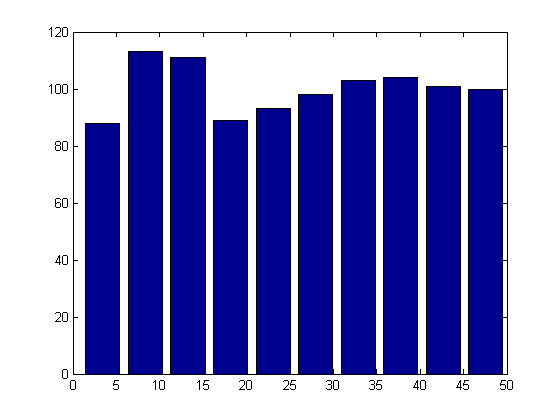
\includegraphics[scale=1]{Figures/1000_agents_color_cluster}
\caption{Color Clusters}
\label{fig:color_clusters}
\end{figure}


Like for any project with a large number of agents, a clear and easy to understand presentation of the simulation was imperative.
Initially, the author went with 2-D histograms depicting the membership values of each color group, which accurately presented how the members move around as the height of the bars representing the number of members in a group could be easily seen to rise or fall, and the speed of this descent or ascent would tell about the rate of success or failure for a particular color. An example could be seen in figure~\ref{fig:color_clusters}.

\begin{figure}
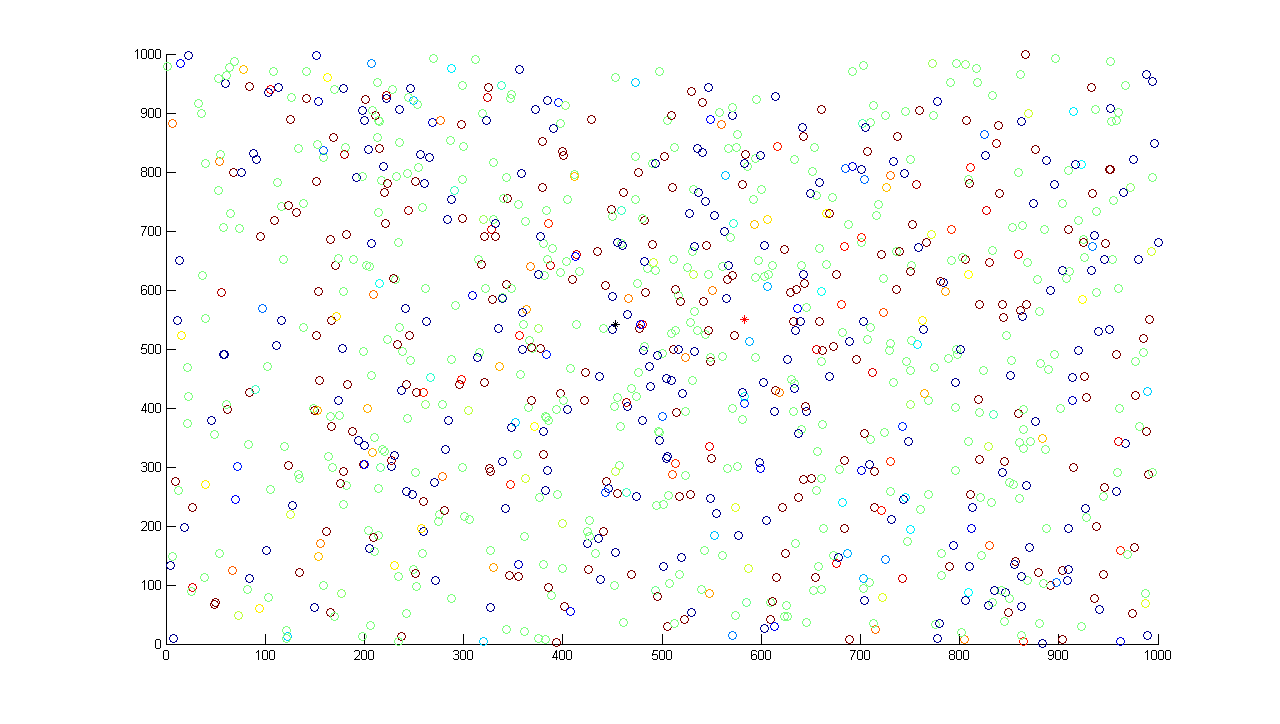
\includegraphics[scale=0.5]{Figures/spatial}
\caption{3-D Spatial Cluster}
\label{fig:spatial_clusters}
\end{figure}



However, with the progress of the model this representation became obsolete as it was unable to represent the aspect of ``Cost" to a company. 
To address this necessity, the author decided to switch to a 3-Dimensional presentation, with X- and Y- axes representing generic movement for agents, and the movement or effort as well as incurred cost for the companies, ad the color, being the 3-rd dimension of the presentation, depicting the value of the attribute. The speed of movement here serves the purpose as the speed of rise/fall in the previous model. An example of this is figure ~\ref{fig:spatial_clusters}.

While the X-Y movement in this model, for the agents, is a correlation, the changing colors as they move represent the agents leaning towards or away from a particular company.

%-----------------------------------
%	SUBSECTION 5
%-----------------------------------
\subsection{Company Policies}
\label{sec:policies}
Different companies may have different policies towards customer involvement. 

The customer involvement continuum followed by the author is influenced by the works of Bodil Sanden~\cite{bodil} and follow the categorization by Ives \& Olson ~\cite{1984}.
These categories are :

\begin{enumerate}

\item[1] No involvement. Users are unwilling or not invited to participate.
\item[2] Symbolic involvement. User input is requested but ignored. 
\item[3] Involvement by advice. User advice is solicited through interviews
or questionnaires.
\item[4]  Involvement by weak control. Users have sign-off responsibility at
each stage of the system development process. 
\item[5] Involvement by doing. A user as design team member or as the
official liaison with the information system’s development group. 
\item[6] Involvement by strong control. Users may pay directly for new
development output from their own budget or the users’ overall
organizational performance evaluation is dependent on the
outcome of the development effort. 
\end{enumerate}

Out of these, this thesis focuses on categories 2 and 5.
These two specific categories were chosen because they represent most dissimilar choices while still avoiding the extreme conditions, which allowed the model to simulate the more probable scenarios.

%-----------------------------------
%	SUBSECTION 6
%-----------------------------------
\subsection{Simulation Approach}

The simulation in this thesis focuses on companies attracting agents towards their cause, and the cost incurred in terms of efforts on the part of the company.
The model witnesses three types of potential interactions : 
\begin{enumerate}
\item[1] Company to Agent interaction 

These interactions are predefined, in a sense that a certain number of agents already seeded to believe in a company at the beginning of the simulation. This is explained further in Chapter ~\ref{Chapter3}.

\item[2] Agent to Agent interactions

These interactions are the means by which one agent may influences another to lean towards a company. In this model, the agents belonging to either of the companies in question are referred to as  \emph{influencing agents}, and the others are referred to as \emph{influenced agents}. This also mimics real life as the connections betweens agents are directional.

\item[3] Agent to Company interactions

Whenever an agent is influenced, during the simulation, this also causes the company to make some effort, the amount of which depends on its policies. These interactions are what cause the cost to the company.


\end{enumerate}

The outcome of these interactions are measured by the following two values:

\begin{enumerate}
\item[a] Gain

This refers to a company successfully influencing an agent to lean towards itself.

\item[b] Cost

This refers to the cost incurred to the company and is a function of the effort made by the company. It depends on the policy being followed by the company.
\end{enumerate}
	





%-----------------------------------
%	SECTION 2
%-----------------------------------

\section{Tools}
As a requirement from the University, Matlab was chosen as the programming language, and no special toolboxes were used.
The curve fitting app was used occasionally to check the output of the simulation.

The formulas, and variants thereof, used by the author were sometimes first tested as a prototype in Python with NetworkX and Mathematica for mathematical validation. However, any of those implementations do not directly contribute to the result.
